\documentclass{article}
\usepackage{multicol}
\usepackage{graphicx}
\usepackage{titling} % pacote para ajustar o título
\setlength{\columnsep}{1cm}
\setlength{\droptitle}{-4cm} % ajuste vertical do título
\usepackage[bottom=3cm]{geometry} % margem inferior de 2cm
\setlength{\parindent}{1cm} % define recuo de 1em
\setlength{\parskip}{12pt} % define espaçamento entre parágrafos como 12pt
\title{Predição de desfecho clínico para pacientes com Leucemia Mieloide Aguda}
\author{João Pedro Moro Bolognini}
\date{} % remove a data

\begin{document}

\maketitle

\begin{multicols}{2}

\textbf{1. Resumo}

A Leucemia Mieloide Aguda (AML) é um tipo de câncer e atinge uma taxa mediana de sobrevida de 12 a 18 meses, esse tempo curto gera uma dificuldade na detecção e prevenção da doença, e dependendo do prognóstico, é necessário mais informações para selecionar o tratamento mais adequado ao paciente e, dessa forma, resulta em um atraso que interfere no tempo de sobrevida do paciente, que pode nem sobreviver até o resultado dessas informações adicionais. Com base nisso, usando métodos de Aprendizado de Máquina, nesse projeto vai ser realizado uma análise profunda dos conjuntos de dados disponibilizados a fim de conseguir predizer a probabilidade de um paciente sobreviver ou não após utilizar do tratamento de uma certa intensidade 

\textbf{2. Introdução}

A Leucemia Mieloide Aguda é o tipo mais comum e agressivo da leucemia [1], o que causa um baixo tempo de sobrevida ao paciente, e por causa disso, quanto antes for o diagnóstico e prognóstico correto, mais cedo o paciente faz o tratamento correto e aumenta suas chances de cura da doença. A Leucemia é uma doença que afeta a medula óssea, lugar onde são produzidas as células-tronco, atingindo as células mieloides, que dão origem às hemácias, aos leucócitos e às plaquetas, componentes sanguíneos, o que explica a agressividade da doença, mas na AML essas células-tronco sofrem mutação, que impede o amadurecimento delas e a consequência é que a medula óssea fica cheia de células doentes, essas mutações podem vir com o nascimento ou ser adquiridas durante a vida. 
No Brasil recentemente foram diagnosticados quase 11 mil casos por ano e cerca de 37\% de todas as mortes causadas por Leucemia foram causadas pela AML.

Como fatores de risco da doença, temos a idade, alterações genéticas, doenças do sangue, exposição a produtos químicos e a altos níveis de radiação, tabagismo e tratamento prévio de câncer.
Para diagnosticar a doença existem os seguintes exames: hemograma completo com diferencial, mielograma, imunofenotipagem, testes genéticos, análise citogenética convencional, exame FISH e teste molecular por PCR ou NGS. A partir dos resultados dos testes genéticos, classifica-se o grupo de risco do paciente: favorável, intermediário e adverso.
Como tratamento tem-se a quimioterapia, terapias alvo e o transplante de medula óssea.

Alterações nas expressões gênicas de alguns determinados genes são comuns nessa doença, e entre eles, os que podemos citar que sofrem de maior porcentagem de mutação são: CEBPA, NRAS, KIT, DNMT3A, FLT3, TET2, KMT2D, WT1, PCLO, ASXL2, KRAS, entre outros.
E é nos genes mais comuns de sofrerem alterações de expressões gênicas que esse trabalho se apoia como base.

\textbf{3. Dados e Pré-Processamento}

No projeto são utilizados 5 bases de dados: os dados clínicos de cada paciente, os dados de mutação gênica de cada paciente, os dados de expressão gênica de cada paciente, o conjunto de dados de treinamento e o conjunto de dados de teste. Nos dados clínicos, cada atributo traz uma informação do paciente, idade, sexo, classificação de diagnóstico da doença, que pode ou não ter relação com a doença. Nos dados de mutação gênica, além do atributo ‘Sample ID’ que é o identificador de cada paciente, os atributos restantes trazem a informação se o gene sofreu ou não mutação. Nos dados de expressão gênica, além do atributo ‘Sample ID’, os outros atributos trazem os níveis de expressão gênica de cada gene. Nos conjuntos de dados de treinamento e teste há o atributo ‘Sample ID’, identificador de cada paciente, nos dados de treinamento há o atributo ‘Overall Survival Status’, se o paciente sobreviveu ou não ao tratamento, nos dados de teste é esperado receber se os pacientes presentes irão ou não sobreviver.
Foram realizados os seguintes pré-processamentos nas bases de dados: tratamento de espaços em brancos desnecessários, seja no nome dos atributos ou nos valores dos conjuntos de dados, tratamento dos valores ausentes, preenchendo eles com a média do atributo que possui o valor ausente, tratamento e remoção das amostras redundantes e/ou inconsistentes e normalização dos dados clínicos.
Além disso, na base de dados clínicos foram removidos os atributos 'Sex' e 'Race', já que estes atributos não auxiliam nada no problema. Foi feito também uma seleção dos genes mais comuns de sofrerem alguma mutação nos dados de expressão gênica e nos dados de mutação gênica, sendo selecionados 116 genes no conjunto de dados de expressão e 46 genes no conjunto de dados de mutação.

\textbf{4. Protocolo Experimental}

Nos dados clínicos existem 11 atributos, dos quais 1 deles é a identificação do paciente, 8 estão relacionados diretamente com a doença e 2 estão ali apenas para trazer informações adicionais, sendo sexo e raça. Nos dados de mutação gênica há 319 atributos, sendo o 1º o identificador do paciente e os demais  são diferentes genes que trazem a informação do gene ter sofrido ou não mutação naquele paciente. Nos dados de expressão gênica há 14713 atributos, sendo o 1º o identificador do paciente e o resto são diferentes genes que mostram o nível de variação na expressão gênica que o gene sofreu. Nos dados de treinamento existem 2 atributos, o identificador do paciente e o classificador do paciente, 0 ou 1. Nos dados de teste existe apenas 1 atributo que é a identificação dos pacientes que se quer realizar a predição se irá sobreviver ou não ao tratamento.

Como são 3 conjuntos de dados que podem ser utilizados para treinar os modelos, foram testados os 3 separadamente, e depois a junção deles, não fazendo o treinamento com os dados de mutação e de expressão pois possuem atributos em comum e isso atrapalha na análise. Também, há como separar algumas features dos dados clínicos que são strings em como features separadas, há também a possibilidade de reduzir a quantidade de atributos relacionados com a doença, e da para fazer junções com essas possibilidades. Nos dados de mutação e de expressão, dá para se usar com todos os atributos e dá para também fazer uma seleção de genes, pegando e separando os genes mais influentes no diagnóstico buscado.

Ao fazer ajustes e diminuir o número de features dos dados de mutação e de expressão gênica, é possível perceber uma melhora no desempenho da predição  do desfecho dos pacientes. Também, ao fazer uma seleção de features nos dados clínicos, é possível ver uma melhora desse desempenho. Com isso, foram explorados diferentes ajustes e analisados para trazer um modelo eficiente.

A curva de aprendizado do Gradient Boosting (Figura 1) mostra que não ocorre sub-ajustamento ou sobre-ajustamento no modelo. Entretanto, isso varia de modelo para modelo, como podemos ver no modelo de Regressão Logística (Figura 2), que apresenta uma precisão alta e constante no conjunto de treinamento e uma melhora na precisão da validação cruzada, porém não tem o mesmo padrão do Gradient Boosting, uma vez que a precisão decai um pouco no final da validação cruzada.

Analisando as precisões e acurácias dos modelos (KNN, Regressão Logistica, SVM, Redes Neurais Artificias, Naive Bayes, Decision Tree, Random Forest, Gradient Boosting, Ada Boost) nota-se que o modelo de Gradient Boosting tem a melhor acurácia entre os modelos(Figura 3). O modelo de Regressão Logística possui uma acurácia bem parecida com os demais, diferenciando-se na curva de aprendizado, que possui uma acurácia alta com poucas amostras como base de treinamento, o que não é visto nos demais. Já em relação as precisões (Figura 4), nota-se que todos os modelos possuem o mesmo valor, o que indica que todos possuem as mesmas proporções de falsos positivos e negativos, verdadeiros positivos e negativos.
\begin{center}
    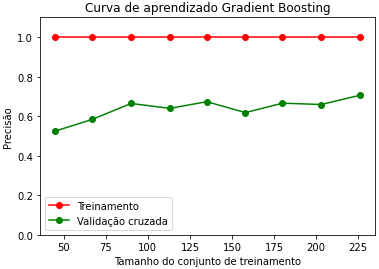
\includegraphics[width=7cm]{Figuras/ca_gb}
    Figura 1: Curva de Aprendizado Gradient Boosting.
    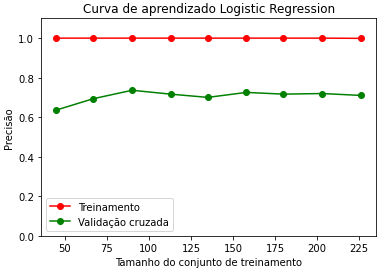
\includegraphics[width=7cm]{Figuras/ca_lr}
    Figura 2: Curva de Aprendizado Regressão Logística.
    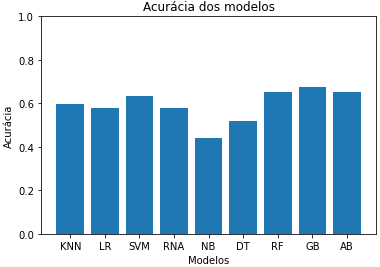
\includegraphics[width=7cm]{Figuras/acuracia_modelos}
    Figura 3: Acurácia dos modelos.

    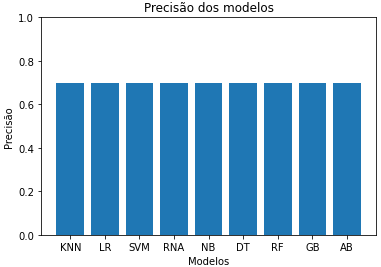
\includegraphics[width=7cm]{Figuras/precisao_modelos}
    Figura 4: Precisão dos modelos.
\end{center}

Devido a esses fatos, esses são os dois modelos escolhidos em decisão final.

\textbf{5. Resultados}

Os desempenhos obtidos no \textit{Public LeaderBoard} na maioria dos testes não teve a acuracia roc semelhante das encontradas no projeto.
Para realisar as análises no projeto, o conjunto de treinamento foi dividido em teste, treinamento e validação.
As 50 últimas amostras foram as de teste e as restantes foram as de treinamento.
Os resultados encontrados no projeto podem ser vistos no gráfico da figura 5.

O melhor resultado obtido no placar público do Kaggle foram para os modelos de Regressão Logística e Redes Neurais Artificiais, dando um resultado de 0.85 em ambos. Mas ao análisar a Figura 5, nota-se um valor bem diferente disso.

A figura 6 traz uma tabela de métricas calculadas do modelo, como além da acurácia e precisão, a revocação, a f1 medida e o erro médio quadrado.

As medidas de revocação e f1 medida estão relacionados a quantidade de verdadeiros positivos e negativos e falsos negativos e positivos, enquanto o erro quadrático médio faz, como o nome já diz, o erro médio entre os valores reais e os valores preditos por cada modelo.
\begin{center}
    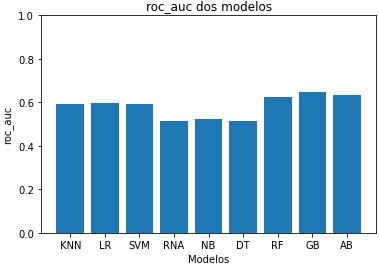
\includegraphics[width=7cm]{Figuras/roc_auc_modelos}
    Figura 5: Acuracia roc de todos os modelos.

    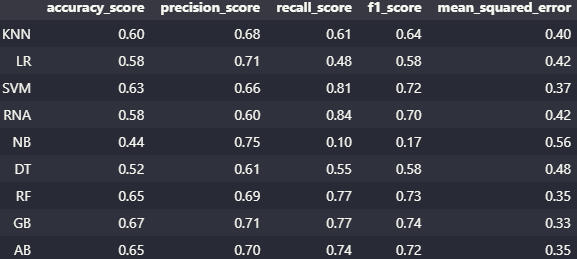
\includegraphics[width=7cm]{Figuras/tabelas_medidas}
    Figura 6: Métricas de todos os modelos.
\end{center}

\textbf{6. Estratégia Final}

As soluções finais utilizam-se da base de dados clínicos, retirando os atributos 'Sex', 'Race', 'Cytogenetic Info' e 'Treatment Intensity', substituindo os dois últimos por uma coluna para cada tipo diferente, tendo quatro intesidades de tratamento, são adicionados 4 novas colunas.
Essa substituição se deve ao fato de como o intuito deste projeto é predizer se o paciente irá ou não sobrevivar ao tratamento indicado, essas duas informações são bem importantes.

Também utilizam-se da base de dados de expressão gênica, pois os níveis de expressão gênicas influenciam no resultado final do paciente, e dessa forma são selecionados alguns genes dos mais de quatorze mil totais, esses genes selecionados tendo uma relação direta com o prognóstico negativo da doença [2].

Estas foram as escolhas finais devido ao fato de com estas duas combinações de seleção de atributos, foram obtidos os melhores resultados no \textit{Public LeaderBoard} e por causa desse bom resultado foram escolhidos estas bases de dados. Vale destacar que não são as melhores para resolução do problema pedido.

\textbf{7. Conclusões}

Este trabalho trouxe diferentes modelos de aprendizado de máquina para predizer se um paciente sobrevive ou não a um determinado tratamento com base nas informações clínicas e gênicas dele.

Os resultados encontrados neste projeto podem não ter cem por cento de precisão e acurácia, mas já indica uma melhora potencial no prognóstico final da doença se o paciente é submetido a determinado tratamento.

\columnbreak

\textbf{8. Referências}

Sites e documentos utilizados para o desenvolvimento deste trabalho: 

[1]https://www.pfizer.com.br/sua-saude/oncologia/leucemia-mieloide-aguda-e-o-tipo-mais-comum-e-agressivo-em-adultos

[2]https://www.jcancer.org/v12p4912.pdf 


\end{multicols}

\end{document}
